We want to do stuff with ion-molecule chemistry and did it

\section{Average Dipole Orientation Theory}

Adiabatic capture theory is a study of the long range potentials between particles to yield a collision cross section, which is then used to calculate a reaction rate constant. This is easily done for many potentials, such as the ion and induced-dipole interaction (Langevin), but is more difficult when considering potentials with another degree of freedom, in particular, we would like to consider the ion-dipole interaction. Unlike the Langevin interaction, the ion-dipole term has a angular term defined with respect to the inter-molecular axis. A few approximations are taken to give an average dipole orientation theory pioneered and expanded on by Su and Bowers.\cite{Su1973, Su1973a} This can also be extrapolated to include quadrupole interactions.\cite{Su1975}

\subsection{Standard Treatment}
A general method of calculating the rate constant of two particles with a given potential, blatantly taken from Willitch.\cite{Zhang2017} The attractive potential is a summation of interactions with coefficient $C_n$ and $r$ dependence $n$.

\begin{align}
    V(r) & = \sum_n -\frac{C_n}{r^n}
\end{align}

In the center of mass frame, we see that

\begin{align}
    V_{eff} & = \frac{l^2}{2 \mu r^2} - \sum_n \frac{C_n}{r^n}\label{eq: veff}
\end{align}

if $n > 2$, we can derive the capture cross section and rate constant as follows. First, we find the position $r_0$ corresponding to the maximum in the effective potential, which is the maximum of the centrifugal barrier.

\begin{align*}
    \frac{\partial V_{eff}(r_0)}{\partial r} & = 0 \\
    \therefore r_0 & = \left(\frac{n \mu, C_n}{l^2}\right)^{1/n-2}
\end{align*}

Substituting $r_0$ back into equation $\ref{eq: veff}$, we find the maximal value of the effective potential:

\begin{align}
    V_{eff}(r_0) & = \left(\frac{l^2}{\mu}\right)^{\frac{n}{n-2}} \frac{n-2}{2n}(n C_n)^{-\frac{2}{n-2}}
\end{align}

This then helps define the energy necessary for a collision, for if $E_{col}$ exceeds $V_{eff}(r_0)$, it will be able to surmount the barrier and react. Thus, we may define the maximum value for the angular momentum $l$ and the impact parameter $b$.

\begin{align*}
    l_{max} & = (\mu n)^{1/2}(C_n)^{1/n} \left(\frac{2 E_{col}}{n-2}\right)^{\frac{n-2}{2n}} \\
    b_{max} & = \frac{l_{max}}{\mu v}
\end{align*}

We can then define a collision cross section dependent on the collision energy:

\begin{align*}
    \sigma(E_{col}) & = \pi b^2_{max} \\
    & = \frac{\pi}{2} n \left(\frac{2}{n-2}\right)^{\frac{n-2}{2}} \left(\frac{C_n}{E_{col}}\right)^{\frac{2}{n}}
\end{align*}

Integrating the collision cross section with a Maxwell Boltzmann distribution yields a generalized rate constant as a function of temperature and n.

\begin{align}
    k(T) & = \int_0^{\infty} v f(v) \sigma(v) dv \label{eq: k int} \\
    & = \boxed{\sqrt{\frac{2 \pi}{\mu}}n\left(\frac{2}{n-2}\right)^{\frac{n-2}{2}}C_n^{2/n}(k_B T)^{\frac{n-4}{2n}}\Gamma\left(2-\frac{2}{n}\right)} \nonumber
\end{align}

\subsection{Ion-Dipole Interaction}

Langevin term of the ion and ion-induced dipole interaction:

\begin{align}
V_L(r)= &-\frac{\alpha q^2}{2r^4}
\end{align}

In the case of the ion-dipole interaction:

\begin{align}
V_D(r, \theta) = & -\frac{q\mu_D}{r^2} \cos(\theta)
\end{align}

The method outlined in section \ref{sec: langevin} finds the rate constant by dealing with a two body problem and only needing to consider the $r$ degree of freedom. The inclusion of the $\theta$ term complicates this, but to first order, we can parameterize it as a function of $r$. What we want to achieve is to write down the potential as such:

\begin{align}
    V(r) =& -\frac{\alpha q^2}{2r^4} - \frac{q\mu_D}{r^2} \cos\left(\bar{\theta}(r)\right) \nonumber \\
    \bar{\theta} = & \frac{\int \theta P(\theta) d\theta}{\int P(\theta) d\theta} \label{eq: avg theta}
\end{align}

Where $P(\theta)$ is the probability of finding the dipole at $\theta$. Two conditions arise:

\begin{enumerate}
\item $P(\theta)$ is inversely proportional to the angular velocity:
$$P(\theta) \propto 1/\dot{\theta}$$
\item An orientation has a probability weighted by the circumference of an angle:
$$C=2\pi l \sin(\theta)$$
$$ P(\theta) \propto \sin(\theta) $$
\end{enumerate}

So then the probability is a combination of the two situations:

\begin{align}
    P(\theta)=&\frac{\sin(\theta)}{\dot{\theta}} \label{eq: prob}
\end{align}

We can relate the angular velocity to the angular kinetic energy and the total energy in the system:
\begin{align}
    KE_{rot} & = \frac{1}{2}I\dot{\theta}^2 \nonumber \\
    E_{tot} & = KE_{rot} + V_D \label{eq: Etot}
\end{align}

Redefining equation \ref{eq: prob} with equation \ref{eq: Etot}, we find:
\begin{align}
    P(\theta) \propto & \frac{\sin(\theta)}{\sqrt{E_{rot}-V_D}} \label{eq: p theta}
\end{align}
%
Combining equations \ref{eq: p theta} and \ref{eq: avg theta} yields:

\begin{align}
    \bar{\theta} = & \frac{\int\frac{\theta \sin(\theta)d\theta}{\sqrt{E_{rot}+q\mu_D/r^2 \cos(\theta)}}}{\int\frac{\sin(\theta)d\theta}{\sqrt{E_{rot}+q\mu_D/r^2 \cos(\theta)}}} \label{eq: avg theta int}
\end{align}

From here, two situations arise:

\begin{enumerate}
\item $E_{rot} = E_1 < \frac{q \mu_D}{r^2}$
There is not enough rotational energy to overcome the dipole locking. The solution is oscillatory, but $\theta$ has a $r$ dependent bound. We let the maximal capture angle be defined as $K$.

$$ E_1=-\frac{q \mu_D}{r^2}\cos(K) $$

When substituted into equation \ref{eq: avg theta int}, we find:

\begin{align*}
    \bar{\theta}_1 & = \frac{\int_0^K \frac{\theta \sin(\theta) d \theta}{\sqrt{\cos(\theta) - \cos(K)}}}{\int_0^K \frac{\sin(\theta) d \theta}{\sqrt{\cos(\theta) - \cos(K)}}}
\end{align*}


After some math (something something integration by infinite series) and get a result of:

\begin{align*}
    \bar{\theta}_1 & = \frac{2 \sqrt{2}A}{\sqrt{1-\cos(K)}} \\
    \text{where }A & \equiv \int_0^{\pi/2} \frac{a^2 \cos(\phi)^2 d\phi}{\sqrt{q-a^2 \sin(\phi)^2}}
\end{align*}

\begin{figure}[H]
\label{fig: theta1}
\centering
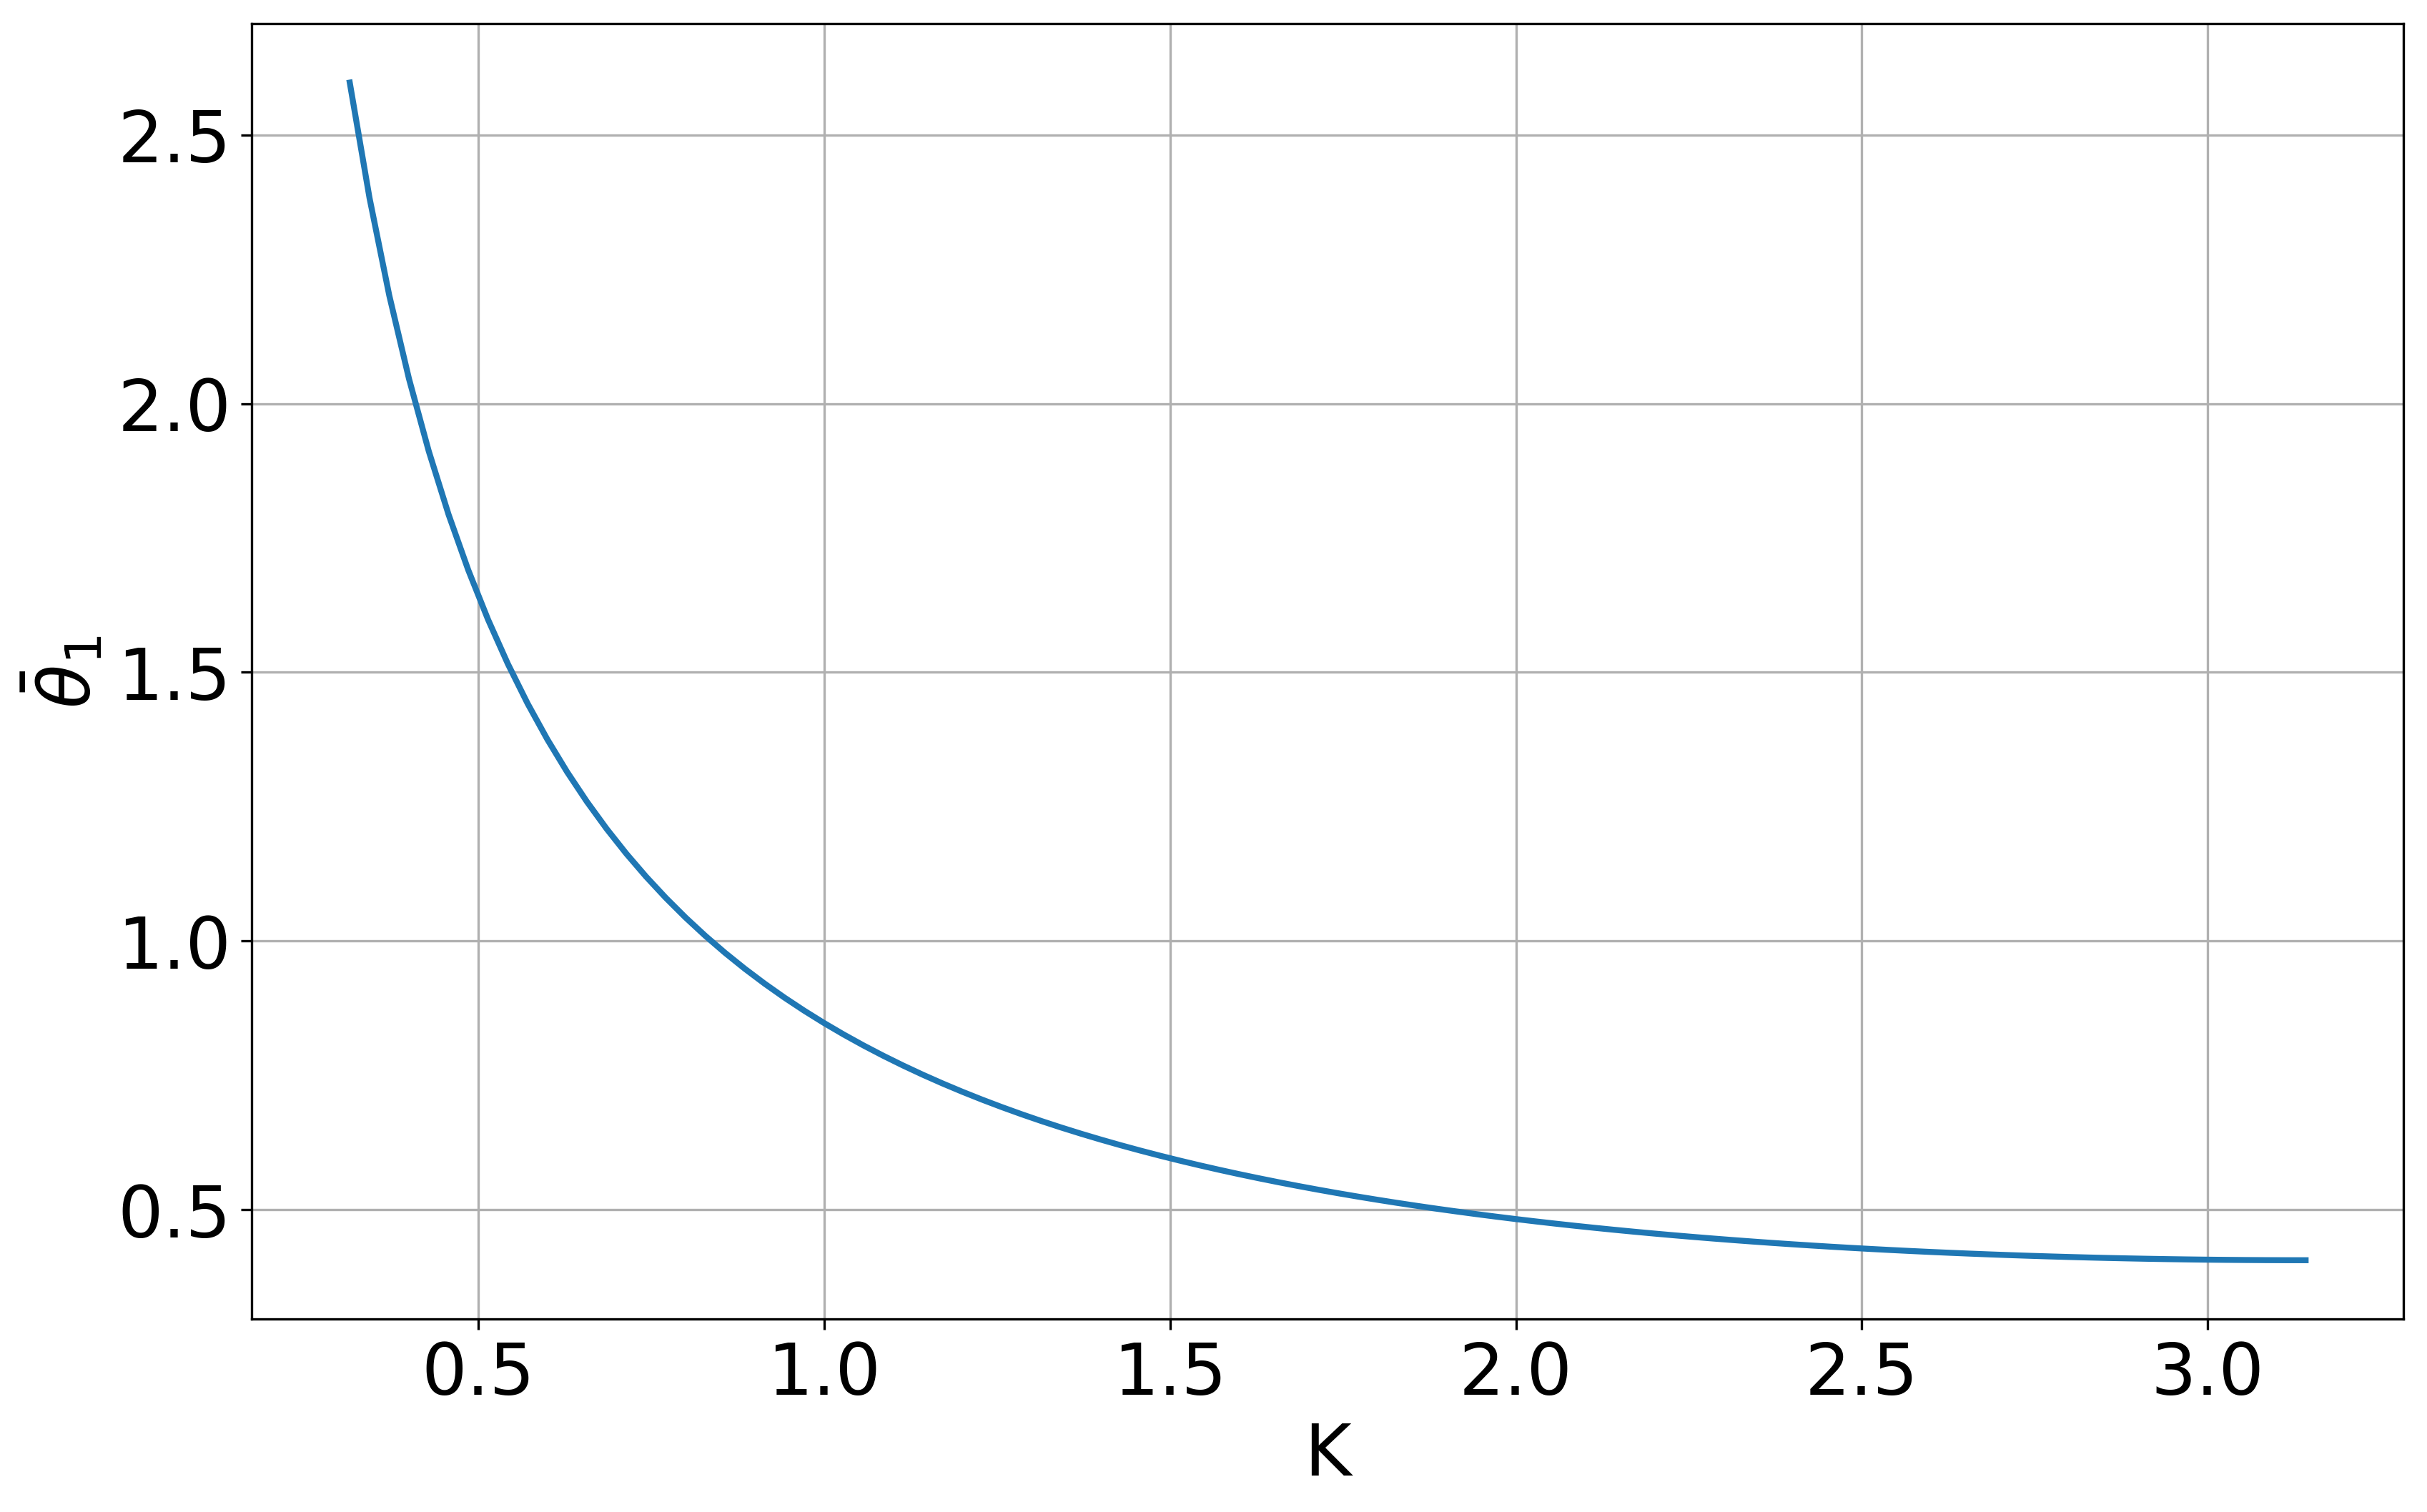
\includegraphics[width=0.8\textwidth]{images/ADO_theta1.png}
\caption{Rough plotting of $\theta_1$ as a function of maximum angle $K$. The behaviour is as expected, the greater the capture angle, the more $\theta_1$ tends towards 0.}
\end{figure}

\item $E_{rot} = E_1 > \frac{q \mu_D}{r^2}$
The rotational energy is enough to overcome the dipole locking and $\theta$ can swing around in a complete circle

\begin{align}
    \bar{\theta}_2 & = \frac{\int_0^\pi \frac{\theta \sin(\theta) d\theta}{\sqrt{E_2 + q \mu_D/r^2 \cos(\theta)}}}{\int_0^\pi \frac{\sin(\theta) d \theta}{\sqrt{E_2 + q \mu_D/r^2 \cos(\theta)}}}
\end{align}

This can be integrated numerically.
\begin{figure}[H]
\label{fig: theta2}
\centering
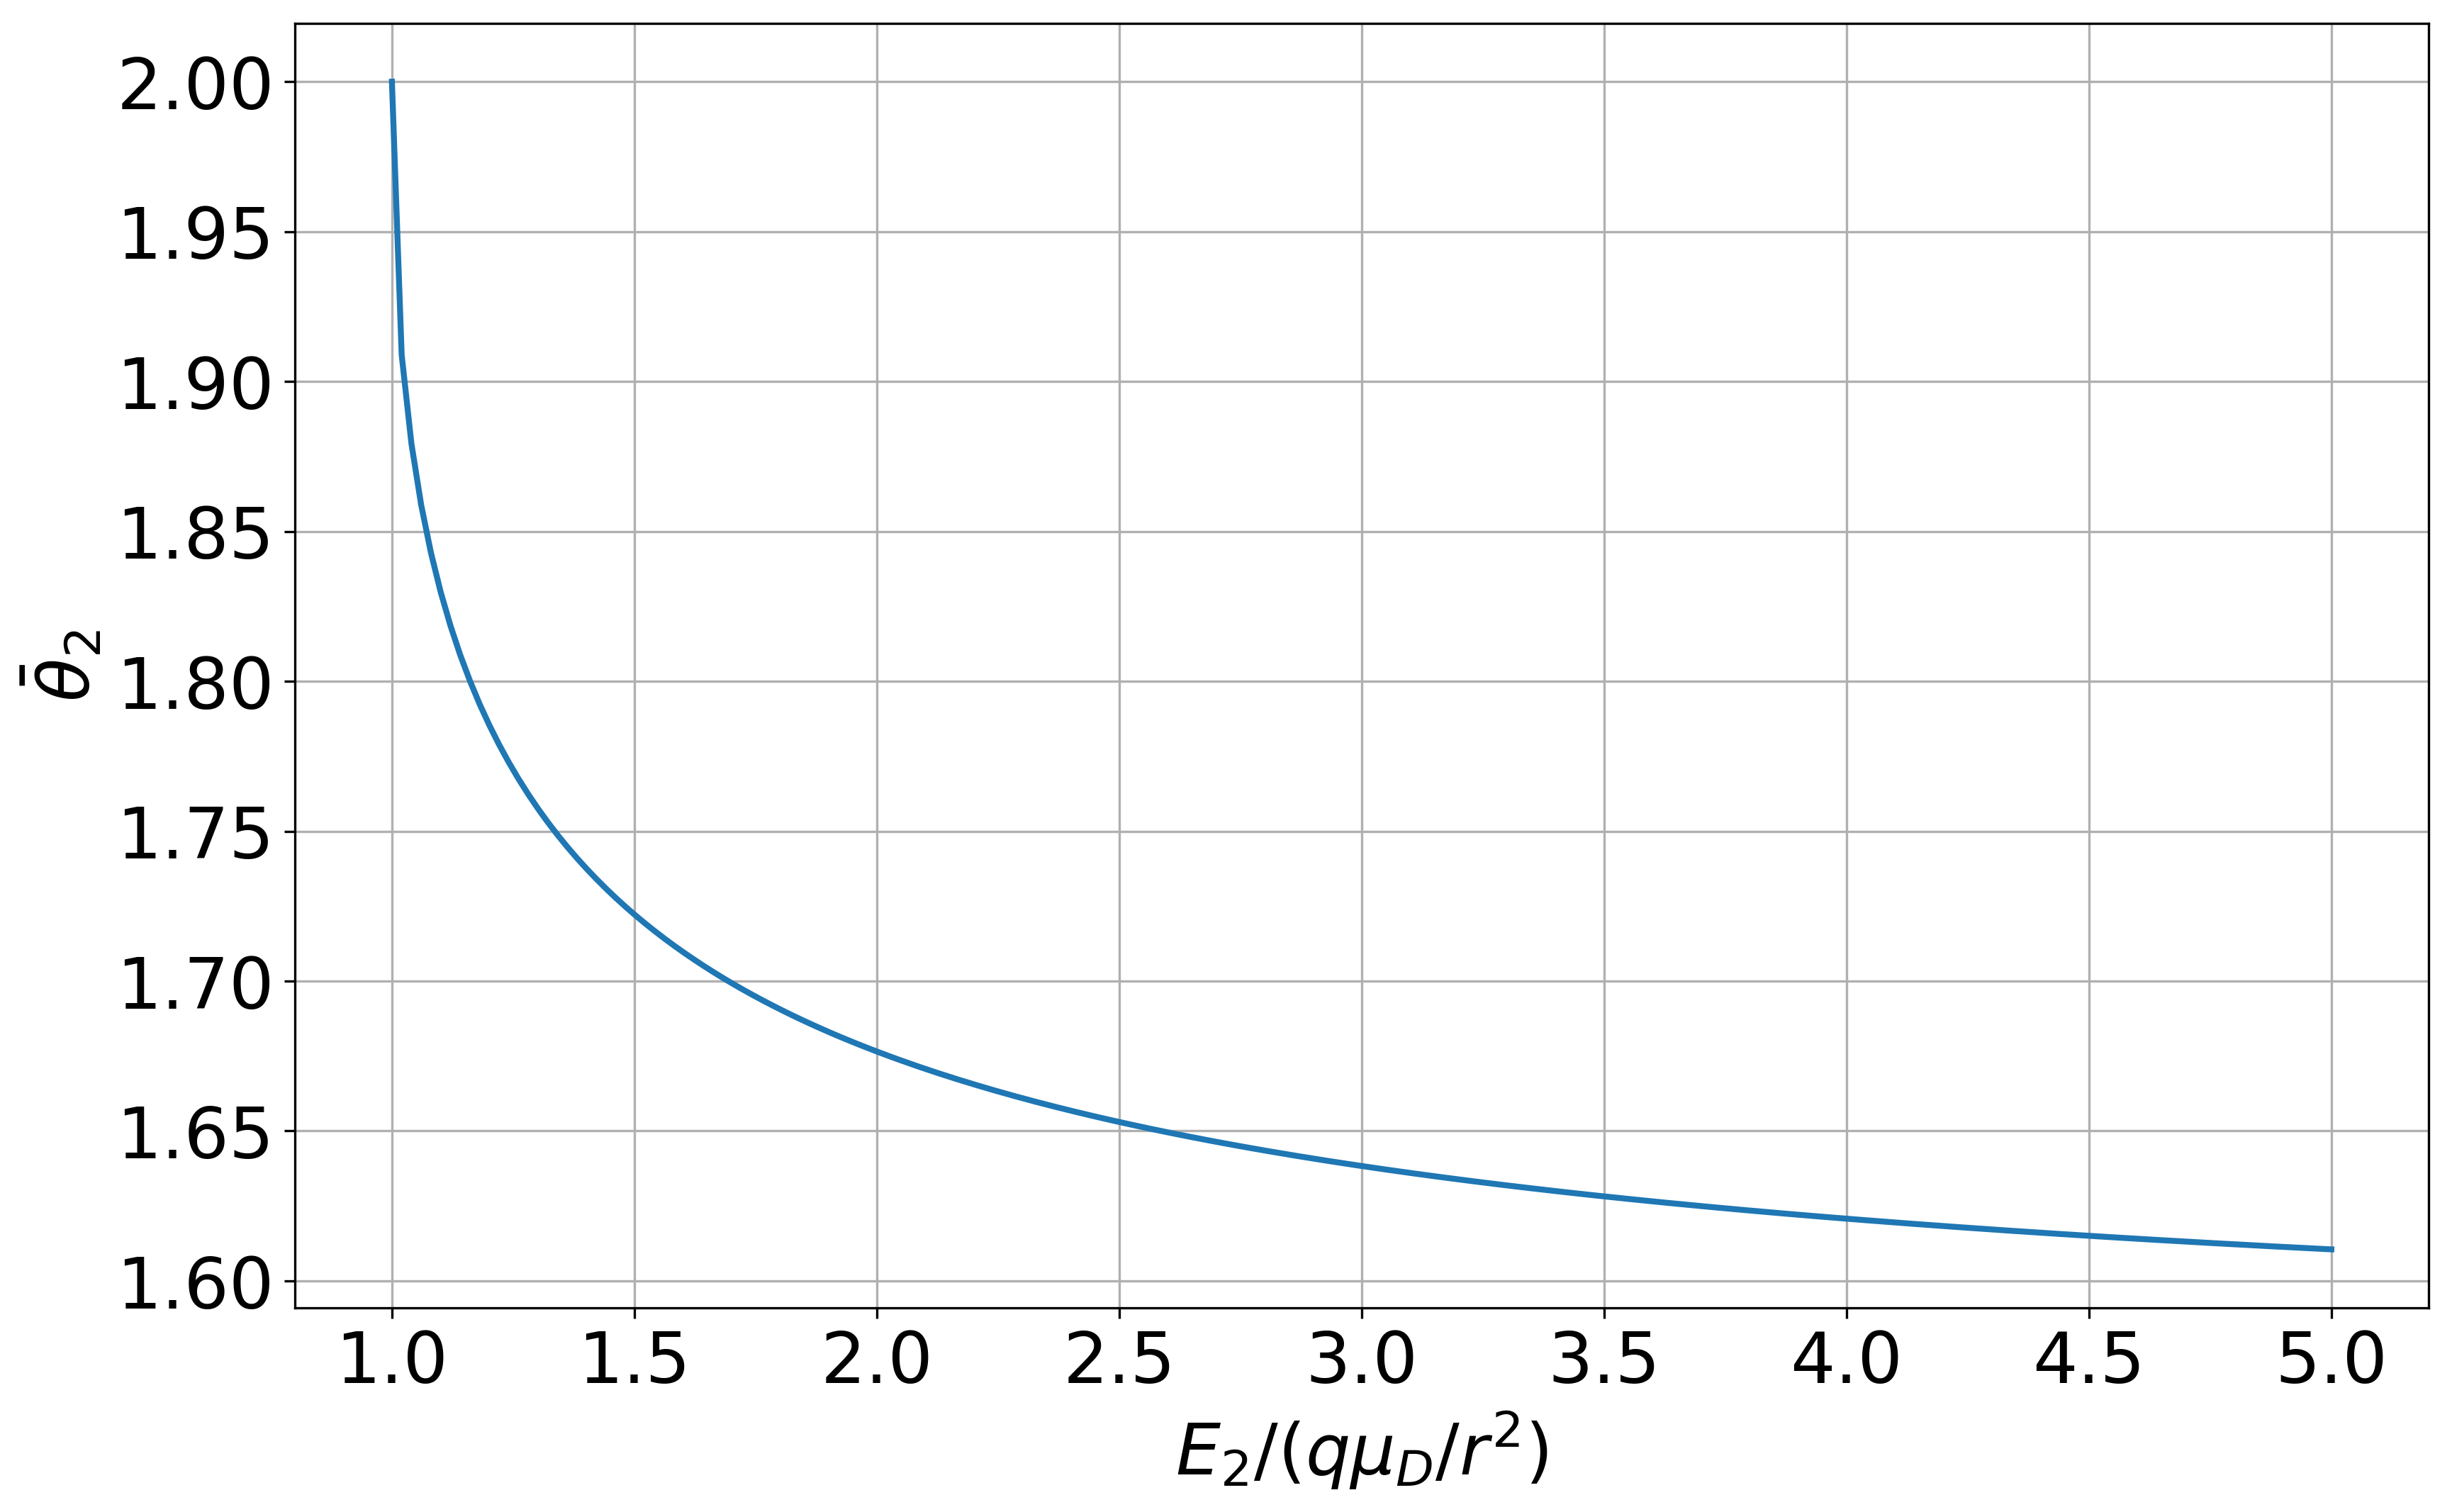
\includegraphics[width=0.8\textwidth]{images/ADO_theta2.png}
\caption{Rough plotting of $\theta_2$ as a function of the ratio of rotational energy and the monopole-dipole term. The low ratio behavior is not immediately obvious, but the greater the ratio between the rotational energy and monopole-dipole term, the more $\theta_2$ tends towards $\pi/2$ (sure).}
\end{figure}

\end{enumerate}

Let's say we have the forms for $\bar{\theta_1}$ and $\bar{\theta_2}$, we want to write down the full form of $\theta$. We can combine the two weighted by the probability of each as a function of internal energy.
\begin{align*}
    \bar{\theta}(r) & = \bar{\theta}_1(r) F_1 + \bar{\theta}_2(r) F_2
\end{align*}

Where these weightings are found via:

\begin{align*}
    P(\epsilon) d\epsilon & = \frac{1}{k_BT}e^{-\frac{\epsilon}{k_BT}}d\epsilon
\end{align*}

For diatomics, we can use:
\begin{align*}
    \epsilon & = \frac{J(J+1)\hbar^2}{2I}
\end{align*}

We can then use equation $\ref{eq: k int}$ and get a cross section and rate constant. The form is similar to that of just a Langevin term, but now with a dipole interaction term added onto it. All of the terms aside from $C$ come from the integration over the Boltzmann distribution, all of the angle averaging is wrapped up into the $C$ term.

\begin{align}
    k_{ADO} = & \frac{2 \pi e}{\sqrt{\mu}}\left(\sqrt{\alpha}+C \mu_D\sqrt{\frac{2}{\pi k_B T}}\right)
\end{align}

The dipole locking constant ($C$) can be numerically solved by iteratively integrating over combinations of $\mu_D$ and $\alpha$, or by looking at figure \ref{fig: C}.\cite{Su1973}\cite{Troe1985}

\begin{figure}[H]
\label{fig: C}
\centering
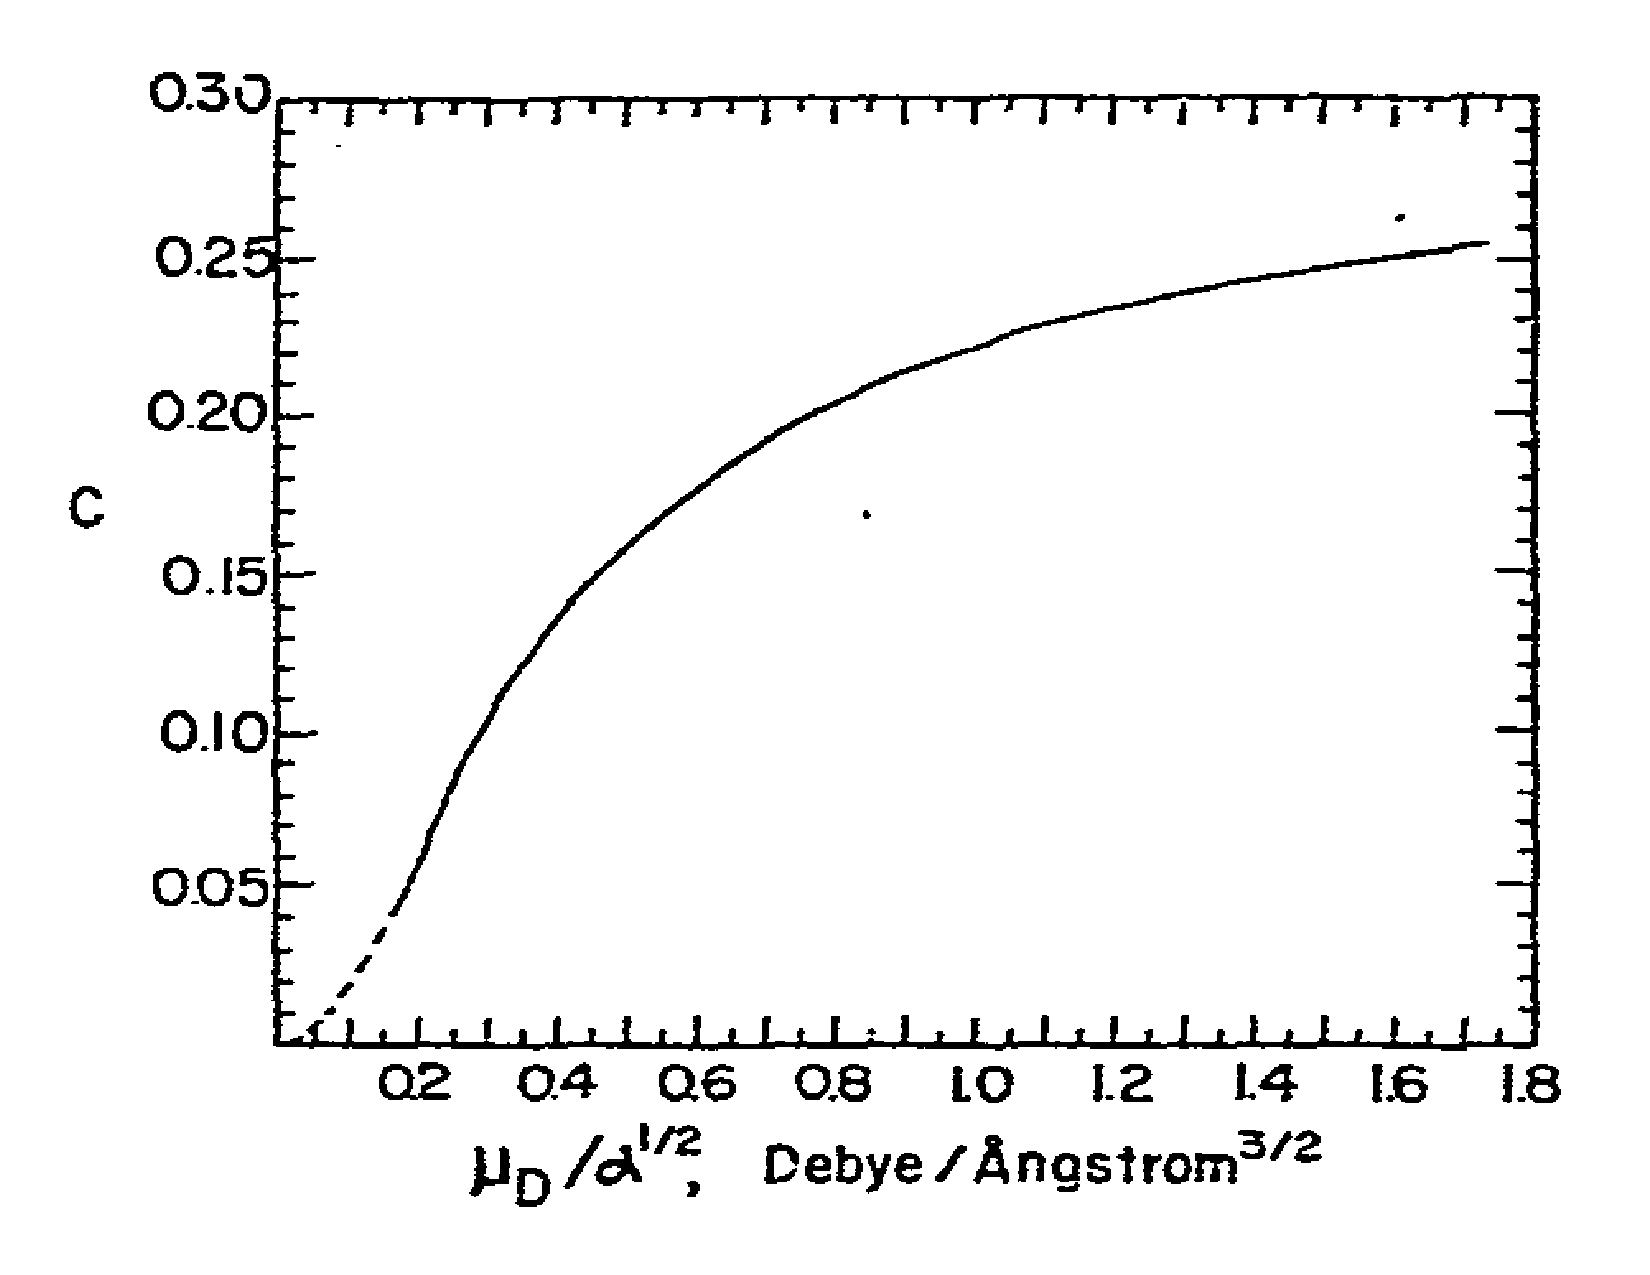
\includegraphics[width=0.8\textwidth]{images/ADO_C.pdf}
\caption{Dipole locking constant $C$ parameterized by the dipole moment $\mu_D$ and polarizability $\alpha$.\cite{Su1973}}
\end{figure}

\section{Introduction to Buffer Gas Beams}

To reach reaction temperatures in the regime of 10K from a beam of molecules with trapped ions, a cryogenic buffer gas beam (CBGB) of neon with entrained water is employed. Numerous methods of creating cold beams of molecules exist, from Zeeman decelerators \cite{Narevicius2008}, Stark decelerators, to cryogenic buffer gas beams (CBGB). CBGB's in particular have the benefit of being species agnostic, where the resultant beam properties are not dependent on the target species at hand, rather, the buffer gas species. \todo{Add citations for decelerators}

By holding a cell filled with a buffer gas of neon of helium above its vapor pressure, a volume of gas can be held at cryogenic temperatures. Other species of molecules are atoms may be introduced into the buffer gas cell via ablation, fill line, etc. The target species particles are then sympathetically cooled via collisions with the cold buffer gas. An aperture at one end of the cell allows for the extraction of the buffer gas and entrained target species into a beam. Regulating the buffer gas cell temperature to above 17K for neon, and 4K for helium, in high vacuum allows us to accumulate an appreciable stagnation number density.
\todo{Add graphic to show what a buffer gas beam is}

The Reynolds number is typically used to characterize the flow regime of the buffer gas beam. At the aperture of the buffer gas cell, the Reynolds number can be written as:

\begin{align} \label{e: reynolds}
Re & \approx \frac{2 d_{aperture}}{\lambda} \\
& \approx \frac{8\sqrt[]{2} \dot{N} \sigma}{d_{aperture} \bar{v}}
\end{align}

Where $d_{aperture}$ is the diameter of the aperture and $\lambda$ is the mean free path of the buffer gas particles \cite{Hutzler2012}.

\subsection{Beam Velocity}

At thermal equilibrium, the velocities inside the buffer gas cell follows a Maxwell Boltzmann distribution:

\begin{align} \label{e: mb_distribution}
f(v) & = \left(\frac{m}{2 \pi k T}\right)^{3/2}4 \pi v^2 e^{-\frac{m v^2}{2 k T}}
\end{align}

Where the mean velocity is:

\begin{align} \label{e: mb_mean}
\bar{v} & = \sqrt{\frac{8 k_B T}{\pi m}}
\end{align}

We may rewrite the distribution as a function of the mean velocity $\bar{v}$ into a simpler form .

\begin{align} \label{e: mb_simplified}
f(v) & = \frac{32}{\pi^2} \frac{v^2}{\bar{v}^3} e^{-4v^2/\pi \bar{v}^2}
\end{align}

To get the velocity distribution in the beam, we can calculate the distribution of particles incident on an aperture in the cell.

\begin{align}
f_{beam}(v) & = \frac{v}{\bar{v}}f(v)  \\
& = \frac{32}{\pi^2} \frac{v^3}{\bar{v}^4} e^{-4v^2/\pi \bar{v}^2}
\end{align}

For low Reynold's numbers (Re<1) the flow at the aperture is purely molecular, which means that there are few to no collisions. This allows us to continue to use the Maxwell-Boltzmann distribution to describe the forward velocity \cite{Hutzler2011c}.

\begin{align}
\bar{v}_\parallel & = \int_0^\infty v f(v) dv \approx 1.2 \bar{v}
\end{align}

The spread of the forward velocity of an effusive beam is the full width half max (FWHM) of the Maxwell-Boltzmann distribution: $\Delta\bar{v} \approx 1.5 \bar{v}$.

As one increases the Reynolds number, one can reach the supersonic regime (Re>100) where the velocity reaches $1.4\bar{v}$ \cite{Hutzler2011c}.

But as the flow regime nears the supersonic regime, forward collisions around the aperture cause boosting of the average velocity as well as a decrease in the velocity spread. Changing the flow regime may also change the ratio of species in the beam as well.

A helium buffer gas held at 4K will be slower than a neon gas held at 17K. Despite this, it is preferable to use neon as a buffer gas due to its ideal cryopumping properties. Helium requires large amounts of activated charcoal, also held at low temperatures, to effectively cryopump. These volumes of charcoal can then become saturated and require purging, limiting one's operating time. Neon on the other hand, only requires a metal surface lower than 17K to create neon ice. The neon ice surface will then act as a cryopump for more neon gas as well, allowing for hours of continuous operation with no appreciable build up of background gas. Our experiment uses neon as a buffer gas for its technical simplicity, the lower achievable temperature with the helium does not yield dramatic gains in the final reaction temperature.

\subsection{Density and Extraction}

The stagnation density inside the buffer gas cell is a function of the physical dimensions of the cell and the number flow rate into the cell. High stagnation densities allows for high densities of reactants at the ion trap center, but can push the beam into an unwanted flow regime where the beam properties are not what one wants. Experimentally, it's preferable to use volumetric flow rates when operating the apparatus, but for calculations, that needs to translate to number flow rate using the ideal gas law:

\begin{align}
\dot{N} = \frac{P f}{k_B T}
\end{align}

where $P$ is pressure and $f$ is the volumetric flow rate, this translates to about $4\times10^{17} \text{ particles} \cdot \text{s}^{-1}$ for 1 SCCM of gas flow. By solving for the number density in the flow out of an aperture with molecular flow, we find that the stagnation density within the cell can be shown as:

\begin{align}
n_{b}=\frac{4 \dot{N}}{A_{aperture} \bar{v}}
\end{align}

In general, buffer gas beams operate with stagnation densities around $10^{15}-10^{17} cm^{-3}$. Outside of the cell, we can describe the density of the beam as a function of distance. \cite{Pauly}

\begin{align}
n(z)=\frac{n_o}{2}\left(1-\frac{z}{\sqrt{z^2+a^2}}\right)
\end{align}

Where $z$ is the distance from the aperture into the vacuum side, $n_o$ is the initial number density, $a$ is the radius of the aperture. In the far field, this goes to

\begin{align}
n(z)=\frac{n_o a^2}{4 z^2}
\end{align}

But there is something that we must consider, that is that we aren't seeing the full aperture while we are at all locations, we are actually seeing an appended area due to the inclusion of apertures and skimmers in the way. So in the calculation for $n(z)$, only $n_o$ has a dependence on the aperture size of the cell, $n(z)$ itself will have a set value defined by the smallest aperture in the beam path.

Sympathetic cooling occurs through collisions between the hot target species being introduced and the cryogenic buffer gas particles. The thermalization of the target species with the buffer gas particles is derived via momentum conservation of hard sphere collisions, where $\approx 10$ and $\approx 100$ collisions are needed to relax translational and rotational states to within a factor of 2 of the buffer gas temperature. Vibrational degrees of freedom may take upwards of $10^4$ collisions to fully thermalize is the elastic collision energy is much lower than the internal vibrational level. By finding the mean free path, we can consider the characteristic length the particles travel to be thermalized with the buffer gas, this is then compared to the characteristic length of the cell to determine the effectiveness of the cooling.

\begin{align}
\lambda = \frac{A_{aperture} \bar{v}}{4 f \sigma \sqrt{m_s/m_b}}
\end{align}

If a species is introduced into the buffer gas cell that has a lower vapor pressure than that is allowed at the current temperature, it will be lost when it comes in contact with the cell walls. The rate of this loss can be described as the  characteristic time of diffusion of a particle in the buffer gas to the physical dimensions of the cell set the diffusion time constant:

\begin{align}
\tau_{diff} = \frac{16}{9 \pi} \frac{A_{cell} n_{0,b} \sigma}{\bar{v}}
\end{align}

where $\sigma$ represents the collisional cross section for the buffer gas with the target species. On the other hand, we have the characteristic pump out time given by the conductance of a cell aperture:

\begin{align}
\tau_{pump}=\frac{4V_{cell}}{\bar{v}A_{aperture}}
\end{align}

By combining the $\tau_{diff}$ with the $\tau_{pump}$, we can get a dimensionless ratio, $\gamma$ that characterizes the extraction fraction out of the cell.

\begin{align}
\gamma = \frac{\tau_{diff}}{\tau_{pump}} = \frac{\sigma f}{L_{cell} \bar{v}} \label{e: gamma}
\end{align}

Notice that the $\gamma$ factor does not depend on aperture size, this is generally true, but increasing the aperture size will lower your number density within the cell, which then influences the characteristic length scale of thermalization. Larger apertures thus run the risk of not allowing your particles to fully thermalize in rotational/vibrational states. But decreasing the aperture size can make alignment as well as controlling the number density more difficult, as finer control over the flow rate is necessary for equivalent flow regimes.